\setcounter{figure}{0}
\setcounter{listing}{0}

\chapter{Work Schedule in Winter Semester \label{cha:chapter1} }



\begin{table}[h]
    \centering
    \begin{tabular}{|c|l|}
    \hline
    \textbf{Semester week number} & \textbf{Info} \\ \hline

    1 & Studying the problem  \\ \hline
    2 & Finding literature \\ \hline
    3 & Finding more sources \\ \hline
    4 & EU AI Act analysis \\ \hline
    5 & Jailbreak analysis \\ \hline
    6 & AI analysis \\ \hline
    7 & Content filter analysis \\ \hline
    8 & Risks of AI solutions analysis \\ \hline
    9 & Experimenting with Jailbreaking \\ \hline
    10 & More experimenting with Jailbreaking \\ \hline
    11 & Evaluating of the experiments \\ \hline
    12 & Document revision and final changes \\ \hline
    \end{tabular}
\end{table}


\begin{refsegment}

% Appendix
% \chapter{Second Chapter}

\say{Here, a quotation is written and even some \say{nested} quotations 
are possible}

\lipsum

Figure \ref{fig:dynabook}:

\begin{figure}[h]
\begin{centering}
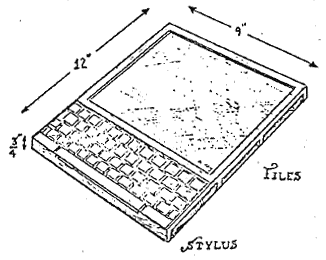
\includegraphics[width=5cm]{assets/images/Dynabook}
\par\end{centering}
\caption{Dynabook \label{fig:dynabook}}
\end{figure}

% Bibliography
\printbibliography[heading=referencessec,segment=\therefsegment,resetnumbers=true]

\end{refsegment}